\title{Arjun Trivedi contribution to NIM pub}
\date{June 05, 2014}

\documentclass[12pt]{article}

\usepackage{hyperref}
\usepackage{cite}

\usepackage{graphicx}
%\usepackage{epsfig}
\usepackage{epstopdf}

\usepackage{mathtools}
\newcommand{\defeq}{\vcentcolon=}

\begin{document}
\maketitle

% \begin{abstract}
% This is the paper's abstract \ldots
% \end{abstract}

\section{III.E. Photomultiplier tubes (PMTs)}

\subsection{Different PMTs time resolutions}
\textit{My assumptions in writing this section}
\begin{enumerate}
	\item \textit{Our chosen PMT(R9779) was compared with panel-1a PMT(EMI9954A)}
	\item \textit {Details of relevant differences of the tech-specs of the two PMTs and therefore the expected superiority of R9779 over EMI9954A will be listed elsewhere; here we will only give empirical proof}
\end{enumerate}

\textit{By the way, can we use the web link directly to Felician's page as a reference? Perhaps not, but this is just to make a note to confirm this.}

The selected Hamamatusu's R9779 PMTs for panel-1b were compared with Electron Tubes EMI 9954A in the 3-bar setup (\textit{I am assuming that the 3-bar setup will either already be defined or referred to in another publication, so as to not go into details, but simply for the reader to trust that it is our way to extract time-resolution, though, it is NOT directly the time-resolution of the PMT, but of the entire counter; this is important to keep in mind, since for the old TOF system, PMT resolutions were directly compared using lasers; details of this method are in old CLAS-SC NIM paper.})

\textit{Should I mention here that for EMI PMT tests, the contribution of the LFIO module was removed?}

\newpage
Below is the figure that shows the superiority of the R9779:
\begin{figure}[th]
	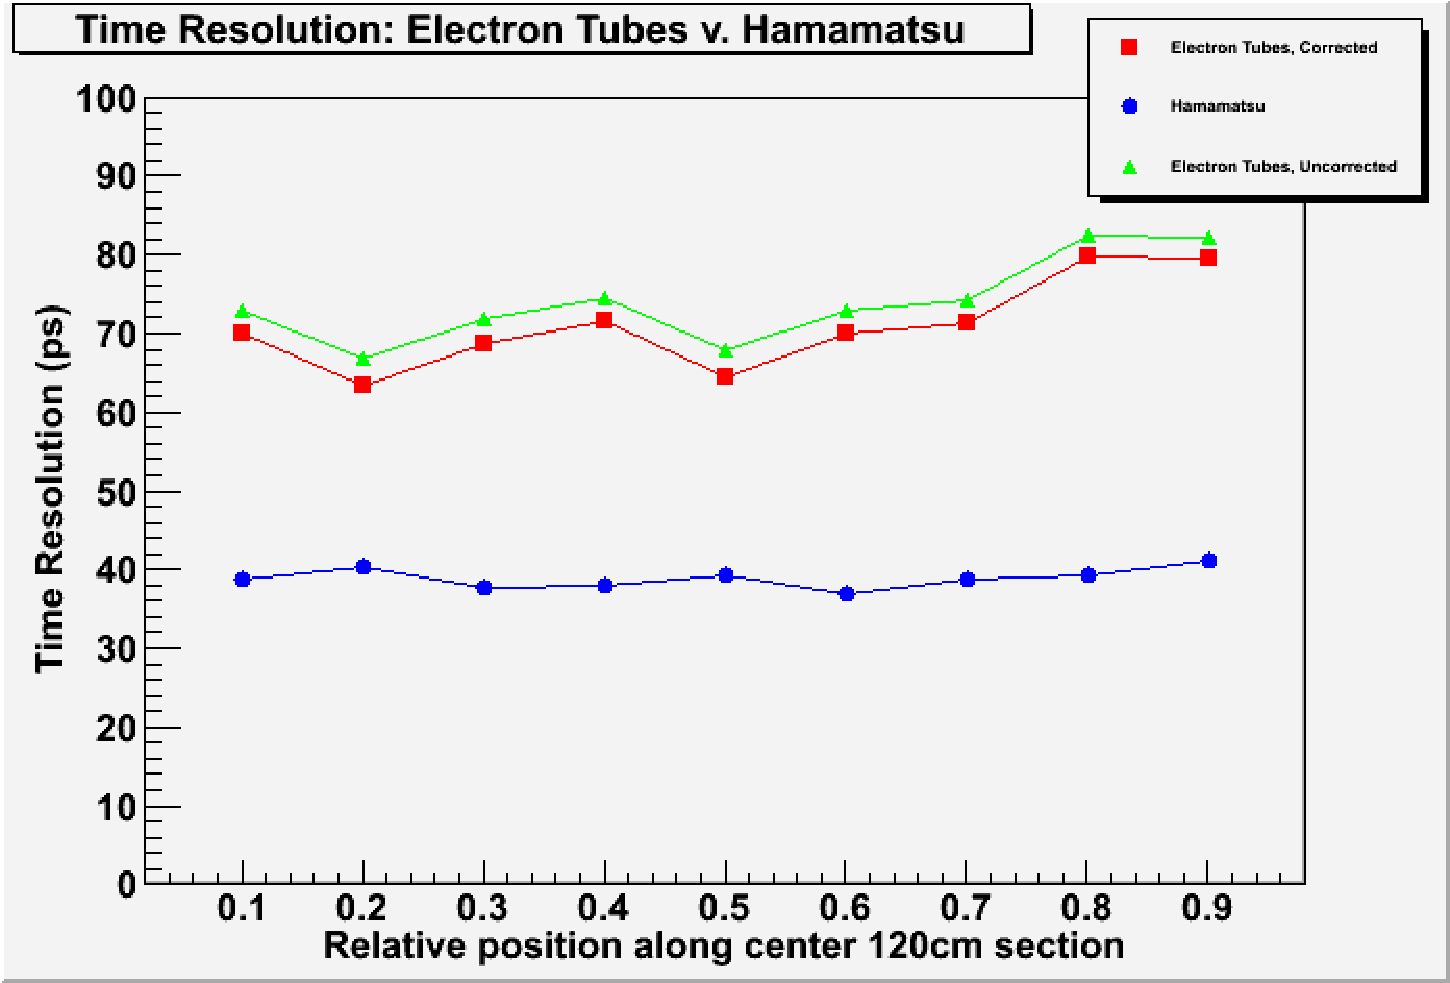
\includegraphics[width=10cm, height=5cm]{PMTcomparison.pdf}
\end{figure}

\subsection{... threshold dependence}
\textit{This section is still lazily written}
We also compared various threshold (\textit{Define "threshold"}) levels for the signals from the PMT and see if it had any affect on the time resolution. The threshold levels tried were:50mV, 75mV, 150mV, 300mV, and 600mV.

Following is a figure that demonstrates varying the threshold did not affect the time resolution.
\begin{figure}[th]
	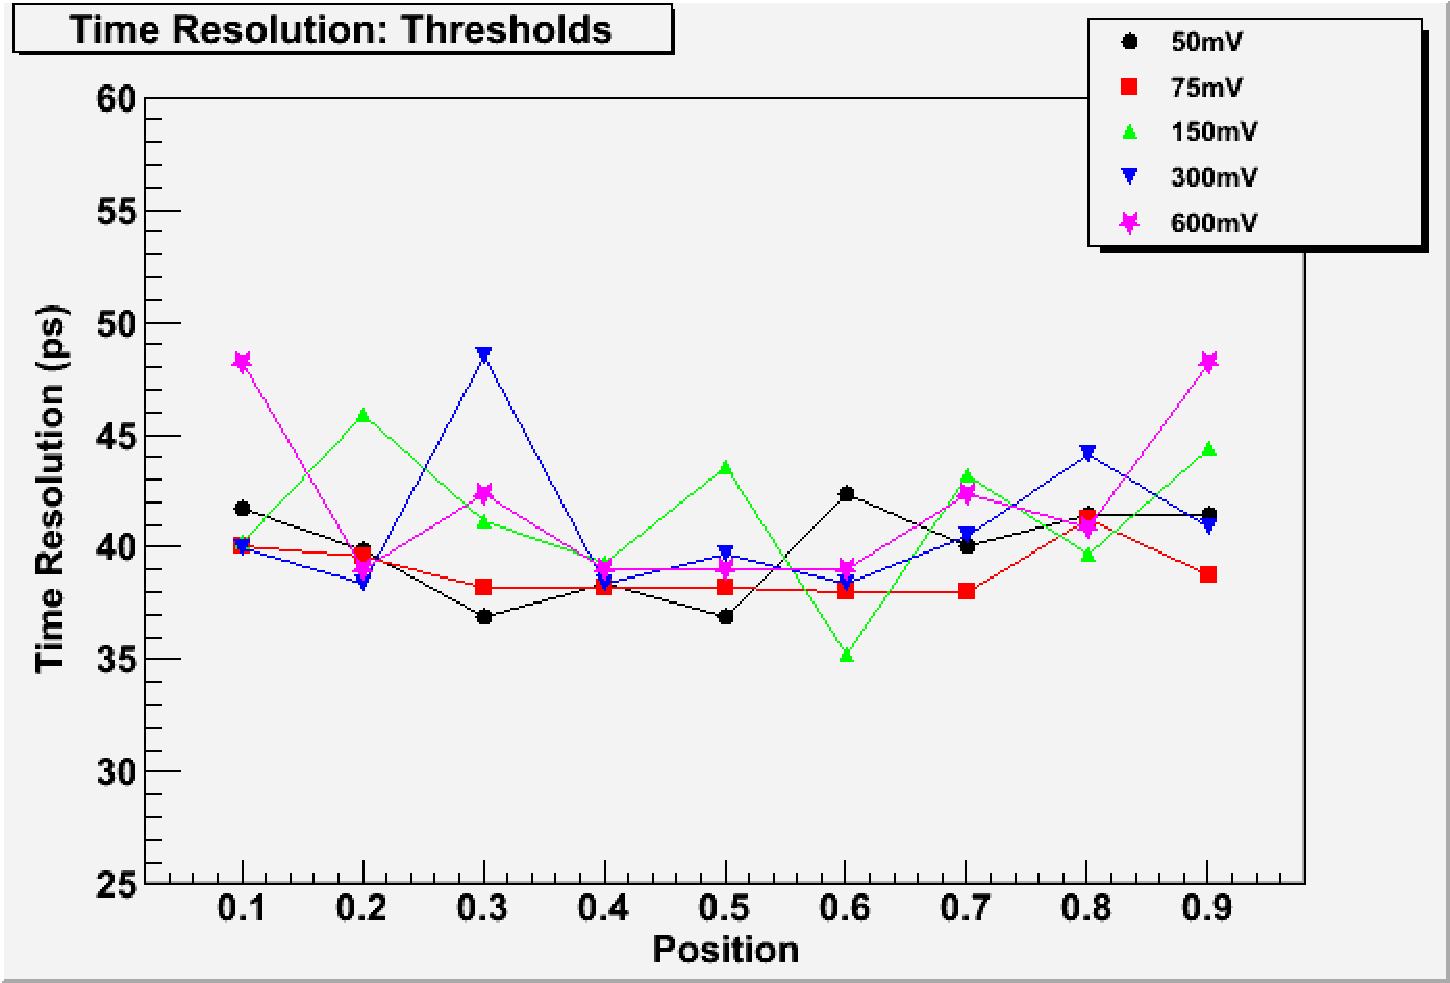
\includegraphics[width=10cm, height=5cm]{ThresholdsTimeRes.pdf}
\end{figure}

\section{III.G. Magnetic shielding}
The PMTs that make up the FTOF counters are going to be exposed to the combined magnetic field from the CLAS12 solenoid and torus magnets. It is therefore important to study the effect of the magnetic field on the signal from the PMT and ultimately, on the time resolution of the counters.

Due to the construction of the PMT and the physical processes which finally contribute to signal formation, the orientation of the PMT relative to the magnetic field is particularly important to note while making observations.  Given a magnetic field, the orientation of a PMT that is constrained to lie on a flat surface, can be described by 2 rotational degree of freedoms. The axes for the 2 rotational degrees of freedom are defined below and illustrated in figureXX:

\begin{enumerate}
	\item $\hat{z} \defeq$ PMT's axis of axial symmetry 
	\item $\hat{r} \defeq$ The axis perpendicular to $\hat{z}$ and the surface
\end{enumerate}

\textit{Illustration figure}

Given a uniform magnetic field, the PMT can be rotated around $\hat{r}$ till it is aligned Transversely or Axially with the field; each of these alignments are defined below.

\begin{enumerate}
	\item Transverse(T): The magnetic field is directed perpendicular to $\hat{z}$
	\item Axial(A): The magnetic field is directed along $\hat{z}$
\end{enumerate}

These are the 2 orientations, under which the PMT is observed to have the 2 strongest, \textit{and in a sense}, 2 independent responses; in any other orientation the PMT's response can be expected to be a superposition of the 2 responses. 

We also studied the additional change in the signal response of the PMT when it was rotated around $\hat{z}$, primarily when the PMT is already aligned in the Transverse orientation(minimal to no effect due to rotations around $\hat{z}$ is expected in the Axial orientation) \cite{Steinman} (\textbf{Re-do measurements:} Steinman has data for rotations around $\hat{z}$ in the Transverse orientation; the fact that there will be minimal impact in the Axial orientation, is what I am hypothesizing). However, after the final shielding implementation, which was mainly designed to protect the PMT in T and A orientations, the PMT response was no longer subject to the additional degree of freedom of rotations around $\hat{z}$.

It is worth mentioning here that the only affect of the magnetic field is on the signal amplitude, while the signal shape, which is the main input for extracting timing information is unaffected \cite{Steinman}. However, the loss of signal amplitude, does affect the extracted time resolution, but only when the reduction is significant. Therefore, in our testing, we directly tested the reduction of signal amplitude and designed the magnetic shielding such that upto levels higher than that expected in CLAS12, the PMT signal amplitude shows no reduction, even though we quantitatively established that for cases when the signal amplitude is reduced by 10\% in the Axial and X\%(\textbf{Measurement of reduction at 20G-T}) in the Transverse orientations there is no change in the time resolution \cite{Steinman}(\textit{I feel like we need to justify this "conservative" approach}). (The maximum field strength that the panel-1b PMTs are going to be exposed to is expected to be 22G, of which 2/3 (15G) will be in the axial direction \cite{CLAS12FTOFstudies}) and we performed our tests with magnetic fields upto 25G wholly directed in either the Transverse or Axial directions.(\textit{actually 30G, but my hesitation in stating so, will be reflected later})

\subsection{Final design and implementation of the magnetic shielding}
To begin with, the PMTs already had a layer of mu-metal coating (\textit{Do we need to be precise here about the thickness of the coating and/or any other important details?}). It can be seen from the following table that compared to a naked PMT, in the Transverse orientation, the inbuilt mu-metal shielding preserved the signal amplitude to much higher levels of magnetic fields.

\textit{Table with following information} \\
no mu-metal: \\
10G-A: 10\% reduction of amplitude (\textit{should clarify that this is actually the mean integrated charge in ADC units, unless I happen to describe the test setup prior to this section}) \\
10G-T: 100\% reduction i.e. complete loss of signal \\
with mu-metal: \\
10G-A: 10\% reduction of amplitude \\
10G-T: 0\% i.e. no reduction \\
20G-T: X\% reduction (\textbf{Quantify reduction?} \textit{Incidentally, both myself and Steinman, only qualitative observed a reduction here, which got worse rapidly as the field levels increased})

Even though at such levels of reduction (\textit{Confirm that at 20G-T, reduction is <= 10\%. I think it is}), the time resolution is unaffected, we decided (\textit{What is the precise argument here, just to be safe? If so, what is the formal name of such an argument, since "just to be safe" sounds amateur-ish}) to add additional, external mu-metal shielding since the magnetic fields in CLAS12 will reach upto 22G, of which 2/3 (15G) will be in the Axial direction \cite{CLAS12FTOFstudies}. 

For the purposes of adding external mu-metal shielding, we chose a rectangular geometry, for this would not only enclose the PMT upto its attachment to the rectangular scintillator bars, but if need be, could also be pushed further, at the cost of shaving off the bars at the edges, to more deeply enclosing the PMT; our testing showed that the deeper the PMT is enclosed in an external shielding, the more it is shielded from Axial fields. The following table demonstrates this fact:

\textit{Table with following information:}\\
(mention thickness of external shielding used here; 2mm for all edges but for the end plate which was 5mm? Perhaps this is not the case, for this additional thickness at the end did not offer much protection in the Axial direction as it was hoped \cite{Steinman}) \\
Show table from log book entry on 1-9-11, where I performed tests upto 5cm depth, upto fields of 30G in the Axial direction. I think it was this table that led to selecting the final overhang/depth to be 4cm. Looking at my table now, I think I can confidently say that, at 4 cm depth, there is no affect on signal amplitude upto 25G in Axial orientation (\textit{perhaps even upto 30G, but I am being extra conservative now})\\
 (\textbf{Redo this measurement?} \textit{Not only would it be a good confirmation if I am indeed being extra conservative, but it may help get me warmed up to redoing Bfield-PMT tests, especially in preparing Nick and getting setup for Breakdown measurement})

 It can be seen that with an external mu-metal shielding and the PMT enlosed to a depth of 4cm, there is no reduction of the signal amplitude in an Axial magnetic field till upto 25G (perhaps 30G); for fields in the Transverse direction, there is no loss of signal amplitude till atleast XX G (\textbf{Breakdown measurement})

 Given the above tests, we decided to enclose our PMTs with inbuilt mu-metal shielding in a rectangular mu-metal box to a depth of 4cm. 

 \subsection{Establishing an upper limit on levels of magnetic field tolerance}
  In the final design of the magnetic shielding, our tests show that there is going to be no reduction in signal amplitude in fields up to 25G (\textit{30G?}) in the Axial and XX G in the Tranvserse orientation. This is already beyond the maximum fields to which the PMTs will be exposed to in CLAS12. However, we did run tests, to note signal reduction factors as we increased the magnetic field beyong 25G/XXG (Axial/Tranverse) and note the point at which the signal amplitude reduced by 10\% and X\% in the Transverse and Axial direction respectively, since we know that upto such reduction factors, the time resolution is unaffected. This would serve as the minimum upper limit of the magnetic field we can confidently state at which the time resolution is unaffected (\textit{This last sentence, again sounds amateurish, but I will leave it as is for now, for it seems like a true statement.}).


\subsection{Results and Conclusions}



% \phantomsection
% \addcontentsline{toc}{chapter}{Bibliography}
\label{bib}
\bibliographystyle{abbrv}
\bibliography{at_contrib}

\end{document}